\documentclass[a4paper]{article}
\usepackage[utf8]{inputenc}
\usepackage[T1]{fontenc}

\usepackage[backend=biber,sorting=none]{biblatex}
\addbibresource{references.bib}

\usepackage{amsmath}
\usepackage{graphicx}
\usepackage{hyperref}
\usepackage{markdown}
\usepackage{placeins}
\usepackage{subcaption}

\title{FYS2085 project work: planetary motion}
\author{Mika Mäki}

\begin{document}
\maketitle
\tableofcontents

\section*{Introduction}
Newtonian gravity simulations are a cornerstone of modern astrophysics.
They can be used to model various astrophysical systems spanning several orders of magnitude all the way from an individual solar system to the movement and merging of galaxies.\footnote{
As a side note they can also be
\href{https://www.kerbalspaceprogram.com/}{highly entertaining} and beautiful to watch but simultaneously \href{https://xkcd.com/1356/}{rigorously rooted in physics}.
}

This project work provides an introduction to such n-body simulations by modeling the Solar System and investingating the effects of different simulation parameters on the results.
Both velocity Verlet and Runge-Kutta 4 integration algorithms are used.

% \href{https://beltoforion.de/en/spiral_galaxy_renderer/}{Approximations}


\clearpage
\section{Methods}
The primary n-body simulator of this project is based on the
\href{https://en.wikipedia.org/wiki/Verlet_integration#Velocity_Verlet}{velocity Verlet} integration algorithm.
Therefore its mathematical basis starts from the familiar Newton's second law
\begin{equation}
\vec{F} = m \vec{a},
\end{equation}
which relates the force $F$ to the resulting acceleration $a$ and the mass of the object $m$.
Using it the acceleration caused by the net effect of multiple forces is
\begin{equation}
\vec{a} = \frac{1}{m} \sum \vec{F_i}.
\end{equation}
Now if we approximate the acceleration to be constant over the time step of interest we have for the velocity and position
\begin{align}
v &= v_i + a_i \Delta t, \\
x &= x_i + v_i \Delta t + \frac{1}{2} a \Delta t^2.
\end{align}
Since these equations are highly prone to divergence due to slight numerical errors, adjustments are needed for better results.
This can be accomplished by averaging the accelerations of the current and previous timesteps, leading us to the Velocity Verlet algorithm
\begin{align}
x_{i+1} &= x_i + v_i \Delta t + \frac{1}{2} a_i \Delta t^2, \\
a_{i+1} &= \frac{F(x_{i+1})}{m}, \\
v_{i+1} &= v_i + \frac{1}{2}(a_i + a_{i+1}) \Delta t.
\end{align}

As this is a Newtonian gravity simulation, the forces between the objects are governed by the
\href{https://en.wikipedia.org/wiki/Newton\%27s_law_of_universal_gravitation}{Newton's law of gravitation}
\begin{equation}
F = G \frac{m_1 m_2}{r^2},
\end{equation}
where $G$ is the gravitational constant, $m_1$ and $m_2$ are the masses of the objects and $r$ is the distance between them.

The second algorithm chosen for this project is Runge-Kutta 4, as it's a very commonly used and versatile integrator with good accuracy.
However, it should be noted that neither the velocity Verlet nor the Runge-Kutta 4 are
\href{https://en.wikipedia.org/wiki/Symplectic_integrator}{symplectic integrators}.
Therefore they both experience a
\href{https://en.wikipedia.org/wiki/Energy_drift}{drift in the total energy}
of the simulated system over time.
The Runge-Kutta 4 algorithm is designed to solve a system of first-order differential equations.
Therefore we have to expand our second-order differential equation to two first-order equations.
These can be written as
\begin{align}
\dot{\vec{r}} &= \vec{v} \\
\dot{\vec{v}} &= \vec{a}.
\end{align}
Now we have two first-order differential equations that can be solved with the algorithm.
However, it should be noted that when computing the intermediate slopes $\vec{k}$, we need to use the intermediate results from the other differential equation that correspond to the intermediate step we are computing.
Therefore we can write the intermediate slopes for the position as
\begin{align}
\vec{k}_{1,r_{i+1}} &= \vec{v}_i \\
\vec{k}_{2,r_{i+1}} &= \vec{v}_i + \vec{k}_{1,v_{i+1}} \frac{h}{2} \\
\vec{k}_{3,r_{i+1}} &= \vec{v}_i + \vec{k}_{2,v_{i+1}} \frac{h}{2} \\
\vec{k}_{4,r_{i+1}} &= \vec{v}_i + \vec{k}_{3,v_{i+1}} h,
\end{align}
where we have denoted the timestep $\Delta t$ as $h$ to be consistent with the usual notation for the algorithm.
The corresponding definitions for velocity are
\begin{align}
\vec{k}_{1,v_{i+1}} &= \vec{a}(\vec{r}_i) \\
\vec{k}_{2,v_{i+1}} &= \vec{a}(\vec{r_i}+\vec{k}_{1,r_{i+1}} \frac{h}{2}) \\
\vec{k}_{3,v_{i+1}} &= \vec{a}(\vec{r_i}+\vec{k}_{2,r_{i+1}} \frac{h}{2}) \\
\vec{k}_{4,v_{i+1}} &= \vec{a}(\vec{r_i}+\vec{k}_{3,r_{i+1}} h).
\end{align}
With these values we can compute the velocity and position for the next step as
\begin{align}
\vec{r}_{i+1} = \vec{r}_i + \frac{h}{6} \left( \vec{k}_{1,r_{i+1}} + \vec{k}_{2,r_{i+1}} + \vec{k}_{3,r_{i+1}} + \vec{k}_{4,r_{i+1}} \right) \\
\vec{v}_{i+1} = \vec{v}_i + \frac{h}{6} \left( \vec{k}_{1,v_{i+1}} + \vec{k}_{2,v_{i+1}} + \vec{k}_{3,v_{i+1}} + \vec{k}_{4,v_{i+1}} \right)
\end{align}

It should be noted that the source used for this algorithm has a typo in the definitions of $\vec{k}_{n,r_{i+1}}$. in its equation 10.
The product between the velocity and the previous $\vec{k}$ should be a sum.
\cite{voesenek_implementing_2008}




\clearpage
\section{Implementation}
The program consists of two parts.
Fortran is used for the computation, and Python for the configuration of the simulation and plotting.
The interface between Fortran and Python is facilitated by
\href{https://numpy.org/doc/stable/f2py/}{F2PY} library, which is nowadays a part of
\href{https://numpy.org/}{Numpy}.
This program also uses several other libraries for plotting.
\href{https://matplotlib.org/}{Matplotlib} is used for exporting static images, and 
\href{https://www.pyqtgraph.org/}{PyQtGraph} is used for 3D graphics and animations.
PyQtGraph in turn is built upon the
\href{https://pypi.org/project/PySide6/}{PySide6} Qt bindings,
and also uses
\href{https://pypi.org/project/PyOpenGL/}{PyOpenGL} and
\href{https://pypi.org/project/PyOpenGL-accelerate/}{PyOpenGL-accelerate} to improve the performance of its 3D graphics.

The program is used through a Python file that contains the specification of the celestial bodies and the selection of tools to analyze the simulation with.
The \texttt{main.py} serves this purpose in this project.
The file \texttt{sim.py} contains the actual simulation wrapper that interacts with the Fortran-based simulation \texttt{core.f90}.

The \texttt{core.f90} Fortran module consists of the primary simulation loop \linebreak \texttt{iterate} and the function \texttt{force} that it uses to compute the forces excerted on an object by the other celestial bodies.
It also contains some printing functions for arrays.
In addition to the Python bindings this module can be called from the Fortran main program \texttt{main.f90}.
This main program utilizes also the modules \texttt{cmd\_line.f90} and \texttt{utils.f90} that provide various utility functions.

The Fortran-based main program can be configured by modifying the ini-like configuration file \texttt{config.txt} in the \texttt{run} folder and passing it as a command-line argument.
The Python-based main program in turn is configured by modifying the values directly within \texttt{main.py}.

Instructions for building and running the program are available in the readme files in the repository.
Copies of those files are included here for convenience in appendix \ref{readmes}.




\clearpage
\section{Results}
At first the software was tested by simulating the binary system of the Sun and Jupiter.
The period is estimated from the average time between the change of sign for the x-coordinate of the orbit.
This gives the results of figure \ref{fig:1a}, and comparing these to the true period gives figure \ref{fig:1a_diff} (parts 1. a) and c)).
In these figures we can see that the simulation starts to rapidly diverge if the timestep is above 0.06 years, which corresponds to about 22 days.
Below this timestep the results are fairly consistent, but with timesteps around 0.05 years it seems that the numerical errors cancel the systematic errors with some timestep values.
Below these timesteps we are left with a systematic difference to the true period.
This could be caused by the integration, but also by differences in the input values and the fact that this does not take into account the effects of general relativity and the gravitational wells of other planets.

\clearpage
\begin{figure}[ht!]
\centering
\includegraphics[width=\textwidth]{fig_1a_1.eps}
\caption{Period of Jupiter's orbit as a function of the simulation timestep}
\label{fig:1a}
\end{figure}

\begin{figure}[ht!]
\centering
\includegraphics[width=\textwidth]{fig_1a_2.eps}
\caption{Difference between the simulated and true orbits}
\label{fig:1a_diff}
\end{figure}

\clearpage
The radius of the orbit of the Sun was also investigated and found to be of the order of $744 000$ km, which is slightly higher than its radius, $696 340$ km.
The error bars denote standard deviation over the course of the simulation.
For the period of the motion of the Sun, please see figures \ref{fig:1a} and \ref{fig:1a_diff}.

\begin{figure}[ht!]
\centering
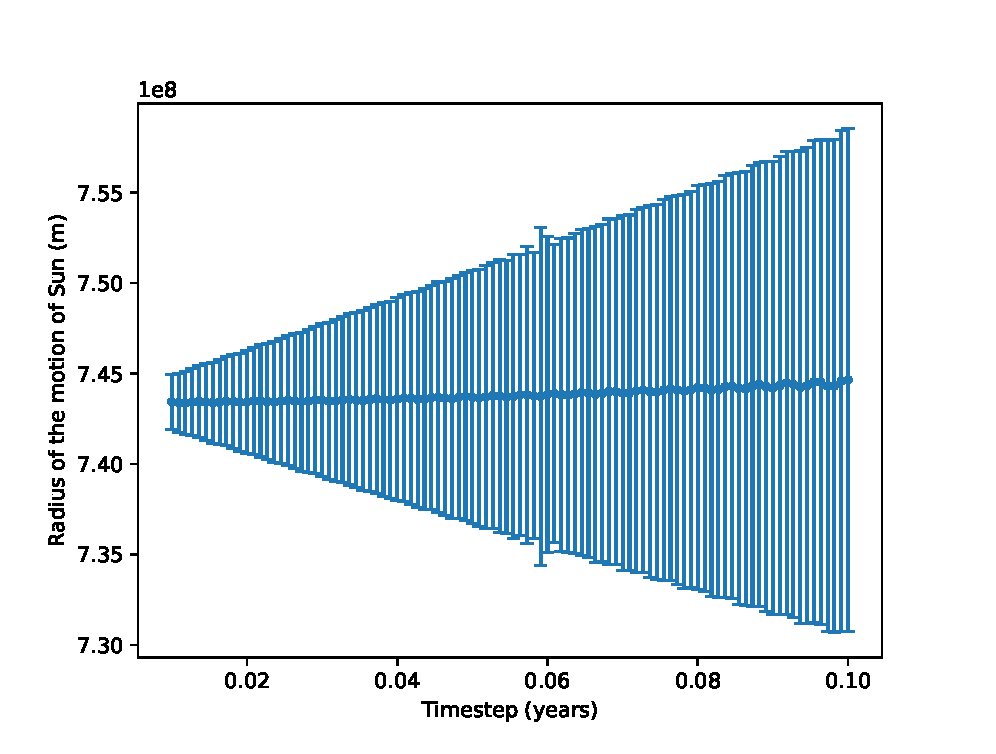
\includegraphics[width=\textwidth]{fig_1a_3.eps}
\caption{Radius of the orbit of the Sun}
\label{fig:1a_diff}
\end{figure}

\FloatBarrier
Then the motion of Jupiter was simulated for one orbital period (part 1. b)).
In this case the reference value for the orbital period was calculated form the initial radius and velocity of its orbit.
According to the results of figures \ref{fig:1b_1} and \ref{fig:1b_2} the movement seems to be too slow compared to the analytical value, but the error is reduced to the order of 1 deg with $10^3$ steps.
However, increasing the number of steps does not reduce the error significantly.
\begin{figure}[ht!]
\centering
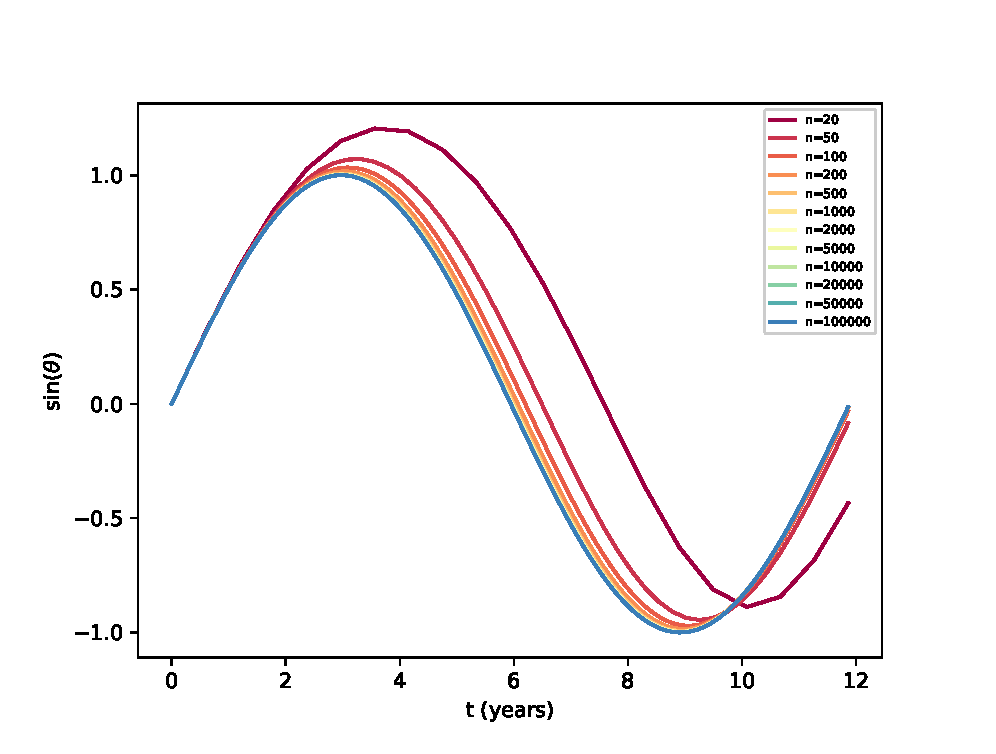
\includegraphics[width=\textwidth]{fig_1b_1.eps}
\caption{Sine of the rotation angle of Jupiter's orbit}
\label{fig:1b_1}
\end{figure}

\begin{figure}[ht!]
\centering
\includegraphics[width=\textwidth]{fig_1b_2.eps}
\caption{Final angle of Jupiter after simulating for one period}
\label{fig:1b_2}
\end{figure}

\clearpage
Other binary pairs were also tested (part 2).
Simulating the length of a year with the Sun and Earth gave the results of figure \ref{fig:2a_2},
and similarly simulating a month with the Earth and the Moon gave the results of figure \ref{fig:2b_2}.
Both of these have a clear point separating a relatively stable solution from a diverging one.
For the simulation of a year this is approximately $dt = 0.05 \ \text{yr}$ and for a month $dt = 0.0004 \ \text{yr} = 0.15 \ \text{d}$.
Interestingly above these values the difference exhibits oscillatory behaviour.

\begin{figure}[ht!]
\centering
\includegraphics[width=\textwidth]{fig_2a_2.eps}
\caption{Relative difference of a simulated year from the true value}
\label{fig:2a_2}
\end{figure}

\begin{figure}[ht!]
\centering
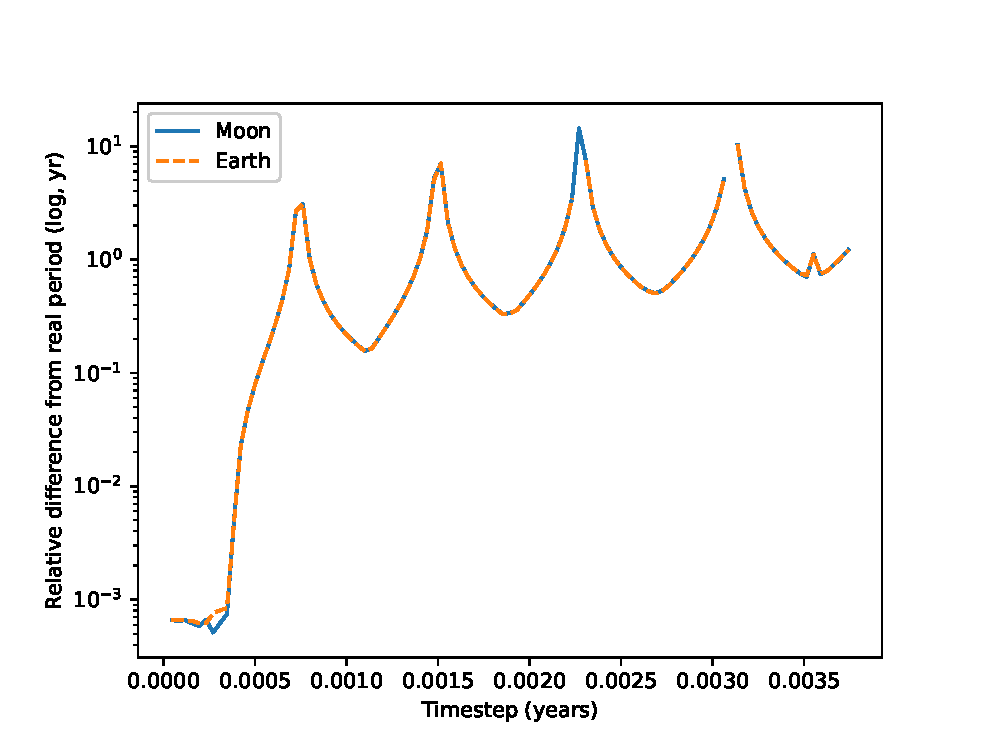
\includegraphics[width=\textwidth]{fig_2b_2.eps}
\caption{Relative difference of a simulated month from the true value}
\label{fig:2b_2}
\end{figure}

\FloatBarrier
As a final test the entire solar system was simulated (part 3), giving the results of figure \ref{fig:3}.
The vertical line corresponds to the $dt = 0.06 \ \text{yr}$, which was the point of divergence for Jupiter in the previous simulations.
It can be seen that the periods of other inner planets are already significantly diverging at these values.
The period of Mercury could not even be computed with the chosen algorithm.
To see where they diverge, we can have a look at the zoomed in version of this plot, figure \ref{fig:3_cut}.
The periods for other planets seem to be relatively stable at around $2 \cdot 10^{-2}$ yr, but for Mercury we need $10^{-2}$ yr for it to be relatively stable.
However, if we look at the zoomed in plot we can see that a step of about $10^{-3}$ yr is needed until the period of Mercury is no longer affected by the choice of timestep.
It should be noted that the lines for the outer planets don't extend all the way to the shortest timesteps, as with those timesteps the simulation ended before they could complete their orbits.

\begin{figure}[ht!]
\centering
\includegraphics[width=\textwidth]{fig_3_rel.eps}
\caption{Relative differences of the orbits compared to their true values}
\label{fig:3}
\end{figure}

\begin{figure}[ht!]
\centering
\includegraphics[width=\textwidth]{fig_3_rel_cut.eps}
\caption{Relative differences of the orbits compared to their true values, zoomed}
\label{fig:3_cut}
\end{figure}

\FloatBarrier
This simulation was also run with Runge-Kutta 4.
Interestingly with this integrator the development of the divergences was not monotonous, but instead with increasing timestep the periods first decrease and then explode.
The overall scale of the timesteps necessary for accurate simulation is similar, but there are notable differences as well.
For Mercury the value explodes at a similar timestep, $10^{-2}$ yr, but when looking at the zoomed plot we can see that the value stabilizes earlier.
This might tempt towards the use of Runge-Kutta 4 over velocity Verlet.
However, Runge-Kutta 4 requires the computing and storage of more intermediate values and seems therefore computationally more demanding.
As is usually the case, each algorithm has its pros and cons.

\begin{figure}[ht!]
\centering
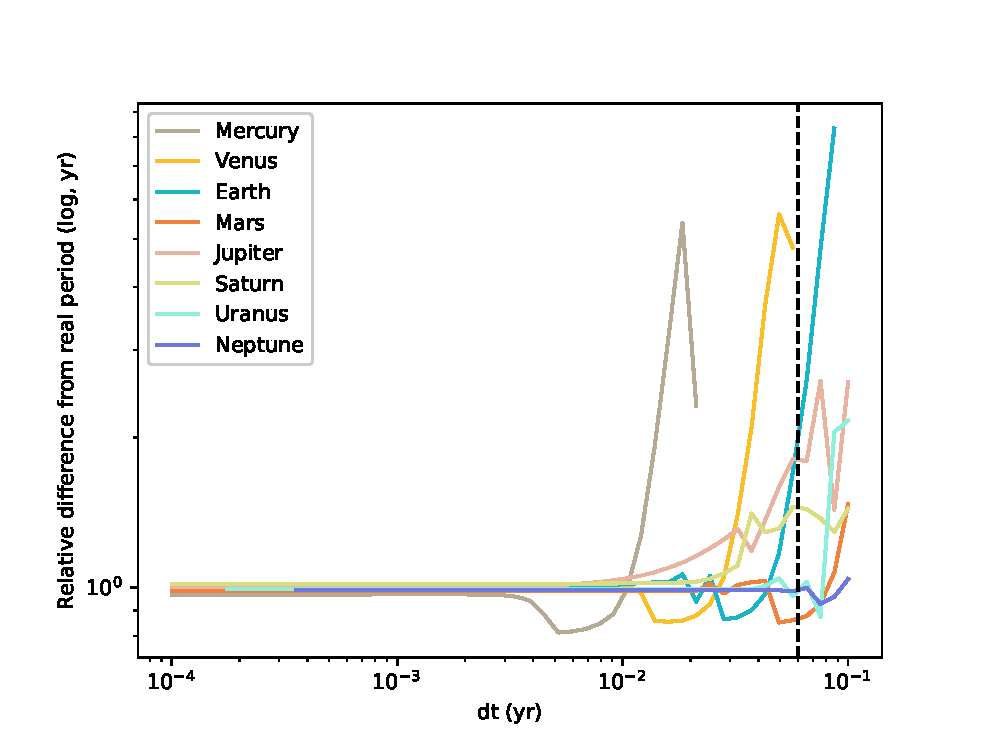
\includegraphics[width=\textwidth]{fig_3_rel_rk4.eps}
\caption{Relative differences of the orbits compared to their true values with Runge-Kutta}
\label{fig:3_rk}
\end{figure}

\begin{figure}[ht!]
\centering
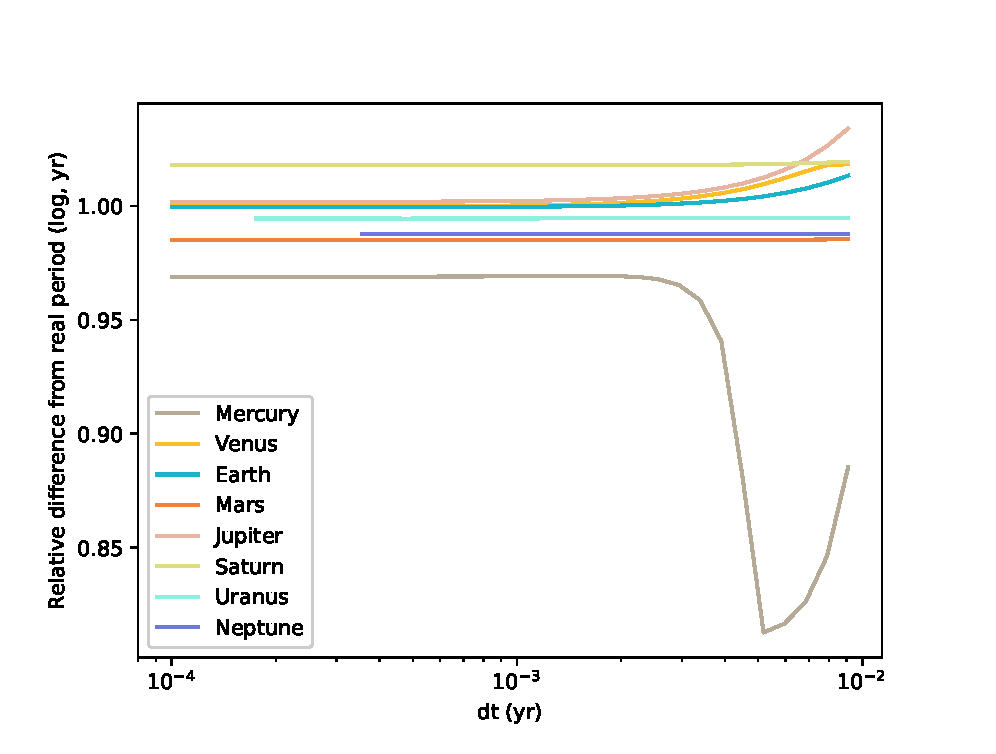
\includegraphics[width=\textwidth]{fig_3_rel_rk4_cut.eps}
\caption{Relative differences of the orbits compared to their true values with Runge-Kutta, zoomed}
\label{fig:3_rk_cut}
\end{figure}

\FloatBarrier
The software also contains tools for interactive 3D visualization.
Please have a look at the commented-out 3D visualizations and n-body simulation tests.
Figure \ref{fig:3d} provides an example of these visualizations.

\begin{figure}[ht!]
\centering
\includegraphics[width=\textwidth]{fig_3d_screenshot.png}
\caption{A screenshot of the 3D visualization}
\label{fig:3d}
\end{figure}


\FloatBarrier
\section{Conclusions}
This project has provided a quick overview to the fascinating world of n-body simulations in astrophysics and a useful template for creating such a simulation.
However, it should be highlighted that neither of the tested algorithms is
\href{https://en.wikipedia.org/wiki/Symplectic_integrator}{sympletic}
and they both will therefore eventually exhibit divergence even with extremely small time steps.
Therefore the most logical continuation to this project would be to implement a sympletic integrator.

Real-world use cases are also extremely large compared to these almost trivial examples.
Therefore for practical applications the performance of the code should be improved significantly, especially with
\href{https://gitlab.com/AgenttiX/tie-51257-project}{parallelization}, as modern supercomputers and even personal computers are nowadays highly parallel systems thanks to the rapid advances in CPU core counts and GPU computing.


\clearpage
\printbibliography

\clearpage
\appendix
\section{Readme files}
\label{readmes}
\subsection{Build and install instructions}
\markdownInput{../src/README.md}

\clearpage
\subsection{Run instructions}
\markdownInput{../run/README.md}

\end{document}
